\section{Introductory Example\label{sec:ch1:example}}

We begin with an introductory design problem that includes decisions that can be classified under the architecture, plant, and control design domains.
This short example will help build some initial intuition for the types of design problems considered here.

\begin{figure}
\centering

\includegraphics[width=0.4\textwidth]{../ch1/figures/robotcontrol_a.pdf}
\caption{Task description in the robotic manipulator example.\label{fig:ch1:robotcontrol_a}}
\end{figure}

% new paragraph
Consider a pick-and-place task shown in Fig.~\ref{fig:ch1:robotcontrol_a} (move an object from one place to another and return) that will be performed by a robotic manipulator (a device that can perform tasks without direct human interaction) \cite{Spong2005a}.
There are a number of ``robots'' that can perform such a task.
A few of these forms or architectures are shown in Fig.~\ref{fig:ch1:robotarch}.
Figure~\ref{fig:ch1:robotarch_a} displays a two-link serial architecture.
An alternative architecture could have an additional link placed in series as is shown in Fig.~\ref{fig:ch1:robotarch_b}.
Links can be combined in a variety of ways to create new architectures such as the four-link parallel manipulator in Fig.~\ref{fig:ch1:robotarch_c}.
Additional components or building blocks can be added to the architectures such as the triangular plate in Fig.~\ref{fig:ch1:robotarch_d}.
There are other decisions to be made with respect to the architecture including the joints that will be active (i.e.,~an actuator is present so a torque can be directly applied to the joint).
The potential actively actuated joints are represented by red arrows in Fig.~\ref{fig:ch1:robotarch}.
From this discussion, the essence of the architecture design decisions is the selection of the components and their connectivity.

\begin{figure}
\centering
\begin{subfigure}[t]{0.22\textwidth}
\centering
	
\includegraphics[scale=1]{../ch1/figures/robotarch_a.pdf}
    \caption{Two-link serial.\label{fig:ch1:robotarch_a}}
\end{subfigure}%
\begin{subfigure}[t]{0.22\textwidth}
\centering
	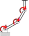
\includegraphics[scale=1]{../ch1/figures/robotarch_b.pdf}
    \caption{Three-link serial.\label{fig:ch1:robotarch_b}}
\end{subfigure}%
\begin{subfigure}[t]{0.25\textwidth}
\centering
	\includegraphics[scale=1]{../ch1/figures/robotarch_c.pdf}
    \caption{Four-link parallel.\label{fig:ch1:robotarch_c}}
\end{subfigure}%
\begin{subfigure}[t]{0.31\textwidth}
\centering
	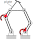
\includegraphics[scale=1]{../ch1/figures/robotarch_d.pdf}
    \caption{Four-link with a plate.\label{fig:ch1:robotarch_d}}
\end{subfigure}%
\caption[Some candidate robot manipulator architectures]{Some candidate robot manipulator architectures (red arrow indicates active joints).\label{fig:ch1:robotarch}}
\end{figure}

% new paragraph
Some potential plant design variables for this problem are shown in Fig.~\ref{fig:ch1:robotplant}.
The link length, cross-section geometry, and ground spacing are all geometric plant variables.
The spacing of the ground joints relative to point $A$ in Fig.~\ref{fig:ch1:robotcontrol_a} could also be considered plant variables.
All of these design variables are time-independent and related to the physical form of the manipulator.
The distribution of the plant variables can vary depending on the architecture considered.
If we use the two-link manipulator in Fig.~\ref{fig:ch1:robotarch_a}, then there will be only two length variables versus the four length variables associated with the four-link manipulator in Fig.~\ref{fig:ch1:robotarch_c}.

\begin{figure}
\centering
\begin{subfigure}[b]{0.33\textwidth}
\centering
	\includegraphics[height=0.5in]{../ch1/figures/robotplant_a.pdf}
    \caption{Link length.\label{fig:ch1:robotplant_a}}
\end{subfigure}%
\begin{subfigure}[b]{0.33\textwidth}
\centering
	
\includegraphics[height=0.7in]{../ch1/figures/robotplant_b.pdf}
    \caption{Cross-section geometry.\label{fig:ch1:robotplant_b}}
\end{subfigure}%
\begin{subfigure}[b]{0.33\textwidth}
\centering
	\includegraphics[height=0.8in]{../ch1/figures/robotplant_c.pdf}
    \caption{Ground spacing.\label{fig:ch1:robotplant_c}}
\end{subfigure}%
\caption{Plant variables in the robotic manipulator example.\label{fig:ch1:robotplant}}
\end{figure}

% new paragraph
The control design could involve the specification of the torque trajectories at the active joints such that the manipulator performs the pick-and-place task shown in Fig.~\ref{fig:ch1:robotcontrol_b}.
These are time-varying signals that could be chosen such that the minimum amount of time or energy is used.
The control design variables directly govern the behavior of the dynamic system.

\begin{figure}
\centering
	
\includegraphics[width=0.35\textwidth]{../ch1/figures/robotcontrol_b.pdf}
    \caption{Joint control trajectories in the robotic manipulator example..\label{fig:ch1:robotcontrol_b}}
\end{figure}

% new paragraph
It is not uncommon for each design domain to be treated separately.
For example, the architecture may be assumed to be fixed while either the plant or control is developed.
Recent work has considered combined plant and control design and this system-focused approach led to low energy consumption solutions \cite{Allison2013d}.
Considering all three of the design domains could further lead to breakthroughs in performance and completely innovative systems.
There are some potential challenges with solving this design problem including the determination of what architectures to consider, developing models for each considered architecture, and solving an appropriate optimization problem for each architecture to properly evaluate its performance.